\section{ATLAS Phase-II升级}
LHC在2020之后会进行一个主要升级,称为High Luminosity LHC(HL-LHC)其将在14 TeV能量下运行,瞬时亮度将达到原始设计目标的5倍$7.5\times10^{34}~\text{cm}^{-2}s^{-1}$,
LHC的计划运行和升级时间表可见图\ref{fig:LHC_timeline}。
HL-LHC的成功运行依赖于超导磁铁等新技术的运用,具体可见HL-LHC技术设计报告\cite{Apollinari:2284929}。
\begin{figure}[h]
\centering
 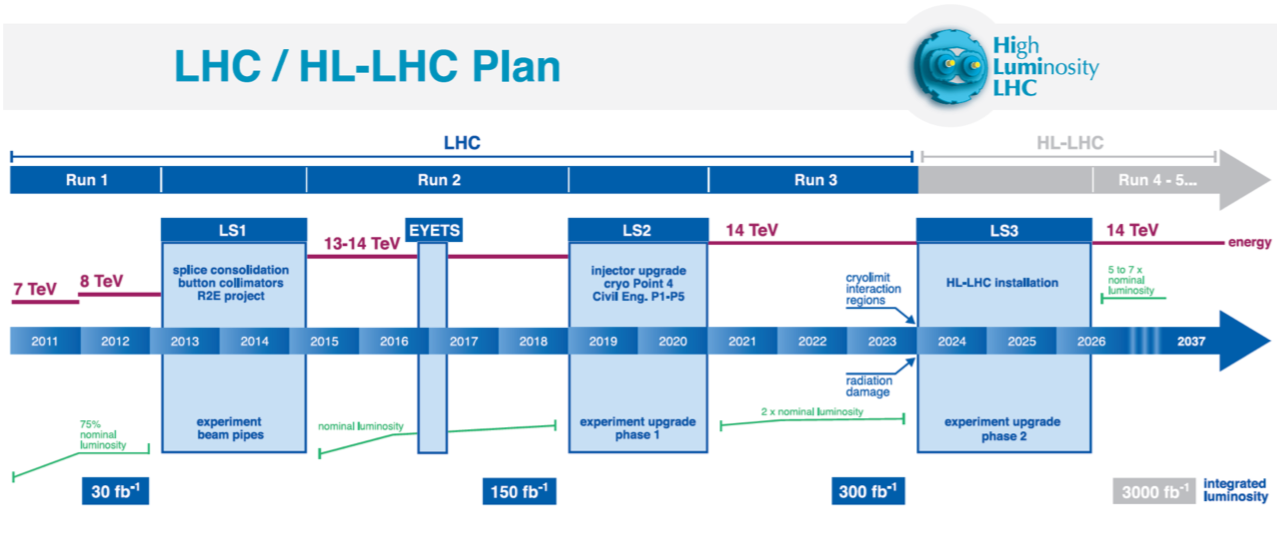
\includegraphics[width=0.85\textwidth]{fig/HL-LHC-PLAN.png}
 \caption{LHC运行和升级时间表\cite{Apollinari:2284929}。}
 \label{fig:LHC_timeline}
\end{figure}
为了承受HL-LHC的高\pileup 和高辐照压力,ATLAS探测器将进行一个全面升级。内部径迹探测器将全部替换成由硅组成的Inner Tracker(ITk),
ITk分为靠近束流的像素探测器(Pixel)\cite{Collaboration:2285585}和扩展到高半径的硅微条探测器(Strips)\cite{Collaboration:2017mtb},Pixel桶部区有五层,Strips则有四层,
一系列环形探测器也会添加到前向区使得寻迹区域扩展到$\abseta<4.0$。
Liquid Argon(LAr)量能器\cite{Collaboration:2285582}将会有全新的前端和读出电子学器件,其电子学架构设计在40 MHz输出全粒度数字信号(full-granularity digitized signals)。
Tile量能器\cite{Collaboration:2285583}会使用新的前端和读出电子学器件,电源和光链路接口板(optical link interface boards)。
$\mu$子探测器\cite{Collaboration:2285580}的一大部分前端,在和不在探测器(on- and off-detector)的读出和触发电子学设备将会被替换,额外的$\mu$子室也会安装以保持$\mu$子的鉴别和重建性能,
另外目前正在研究扩展到$\abseta<4.0$的可能性。
全新的触发和数据接收系统\cite{Collaboration:2285584}也会应用在升级ATLAS上。
考虑到HL-LHC的高pileup,一个新的探测器High-Granularity Timing Detector(HGTD)\cite{Collaboration:2623663}会安装在LAr量能器之前,覆盖$2.4<\abseta<4.0$区域,它可以精确测量带电粒子的时间分辨。
本章将关注硅微条探测器模块和ITk的预期寻迹性能研究。

\subsection{Strips模块组装及测试}
ATLAS Phase-II升级之后的硅微条探测器传感器覆盖165 m$^2$,桶部区有四层,而端部磁盘区有6层,总共需要建造18,000个基本探测模块(module)。一个完整模块由一个
硅传感器,两块或一块包含读出芯片(ABC130Star chip)以及控制芯片(HCCStar)的支撑电路板(hybrid)和电源控制模块(Power Board)组成,具体可见图\ref{fig:strips_module}.
虽然Strips硅传感器的大小和形状根据模块在探测器的位置决定(见图\ref{fig:strip_sensor_overview}),但是其整体设计和架构是一致的。读出芯片是二元设计(binary design),与每条strip通过
金属线相连,信号通过芯片初步处理之后传输到控制芯片,然后统一输出到读出系统,控制芯片同时负责传输控制命令,而电源控制模块则是用来控制整个模块的电源开关以及监控环境参数,各部分的具体
信息可见设计报告\cite{Collaboration:2017mtb}。本文将呈现整个模块的组装过程以及测试结果,所使用的芯片和控制芯片分别称为ABC130和HCC,具体区别同样可见\cite{Collaboration:2017mtb}。

\begin{figure}[h]
\centering
 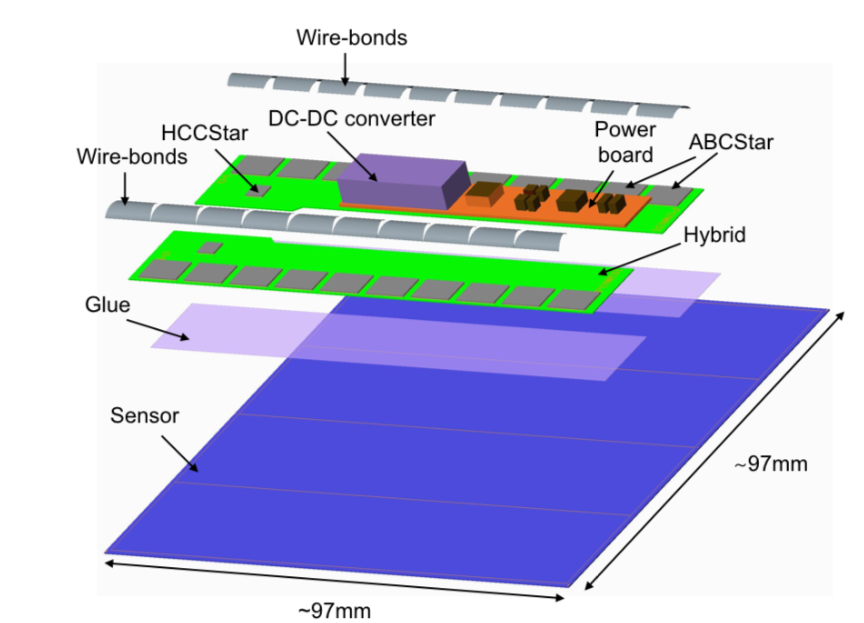
\includegraphics[width=0.85\textwidth]{fig/strips_module_3d.png}
 \caption{(short-strip)Strips模块。}
 \label{fig:strips_module}
\end{figure}

\begin{figure}[h]
\centering
 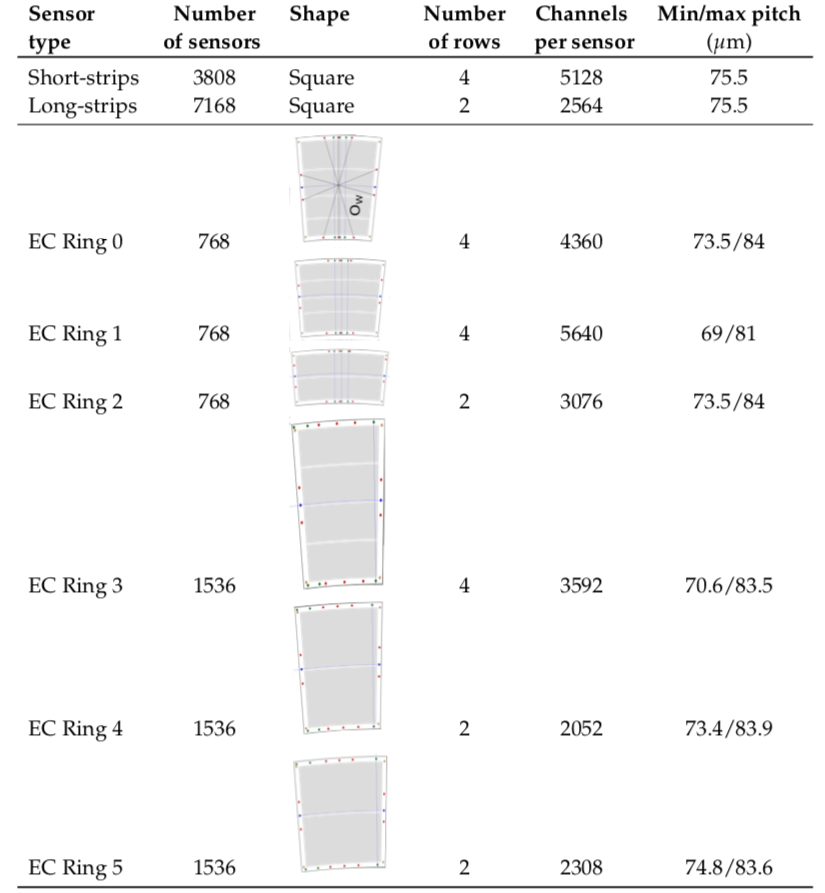
\includegraphics[width=0.85\textwidth]{fig/strips_sensor_overview.png}
 \caption{ITk Strips传感器种类\cite{Collaboration:2017mtb},Strips探测器桶部区内两层由短条(short-strip)传感器组成,外两层由长条(long-strip)组成,由于端部的扇形几何结构,其strip间距(pitch)随半径不同而不同。}
 \label{fig:strip_sensor_overview}
\end{figure}
模块的组装是探测器建造的重要一环,模块的质量决定了最终探测器的性能。
组装过程大致可以分为以下几步:
\begin{enumerate}
 \item 将读出芯片通过胶水粘合在hybrid的相应位置,而后连接读出芯片与hybrid(wire-bonding);
 \item 将芯片通过胶水粘合在传感器上,而后将每条strip与读出芯片相连;
 \item 最后粘合电源控制模块到传感器上,最后进行wire-bonding。
\end{enumerate}
其实际对应过程可见图片\ref{fig:strip_moduel_assembly}\footnote{过程中的具体粘合方法,所使用的器械以及工艺等,一直在进行优化,不同组装地点也可能使用不同的方法。}。
组装的挑战在于各个部分的接触面大小,胶水厚度以及位置的精确控制,一般要求控制到$\mathcal{O}(10)~\mu\text{m}$水平,比如芯片与hybrid的胶水粘合面应当保证至少50\%的接触面,
以便传导芯片工作时产生的大量热量,而固化的胶水应当保持在120$\pm40~\mu\text{m}$厚度。
\begin{figure}[h]
\centering
 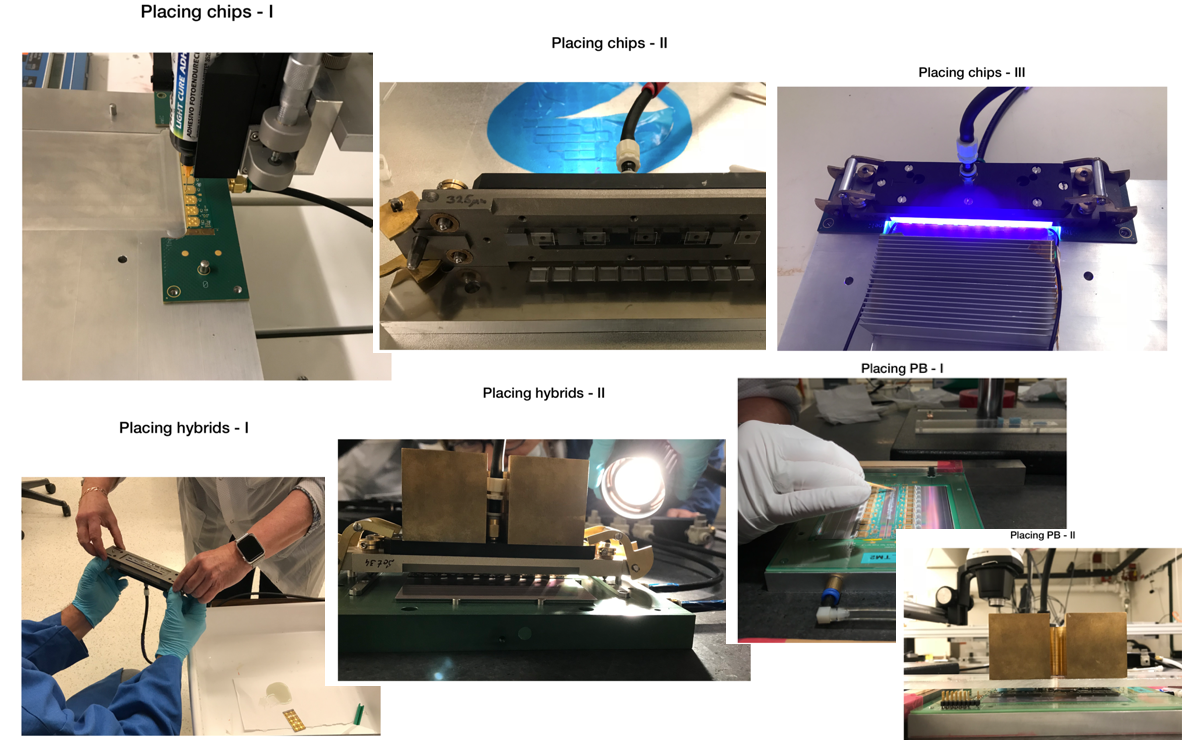
\includegraphics[width=0.85\textwidth]{fig/strips_module_assembly.png}
 \caption{ITk (short-strip)模块实际组装过程(省略wire-bonding过程),粘合芯片的胶水需要紫外线照射固化。}
 \label{fig:strip_moduel_assembly}
\end{figure}
组装完成的模块需要进行电子学测试,以保证模块工作性能达到预期。测试时,模块应当处于干燥且低温的环境中,其测试系统如图\ref{fig:strips_testing_setup}所示。
一个重要指标是衡量ABC130芯片的输入噪声(input noise),它由芯片本身和与之相连的strip噪声决定。
其测试基本原理是给定注入电荷,进行阈值扫描,确定输入噪声水平。图\ref{fig:strips_testing_noise}展示
几个模块粘合PB之前和之后的输入噪声水平,基本在600电子与900电子之间(模块经受辐照之后,整体噪声会上升)。图\ref{fig:strips_bad_dist}则为测试模块的
工作不良strip的空间分布。总体而言,所示的组装模块均工作良好,达到预期。
\begin{figure}[h]
\centering
 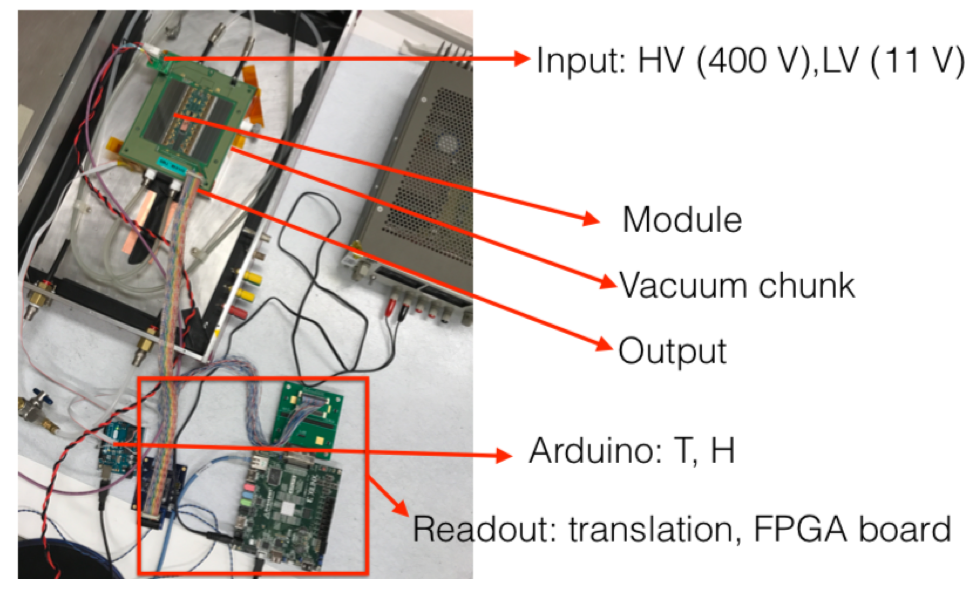
\includegraphics[width=0.85\textwidth]{fig/strips_module_setup.png}
 \caption{Strips模块测试系统设置。}
 \label{fig:strips_testing_setup}
\end{figure}
\begin{figure}[h]
\centering
 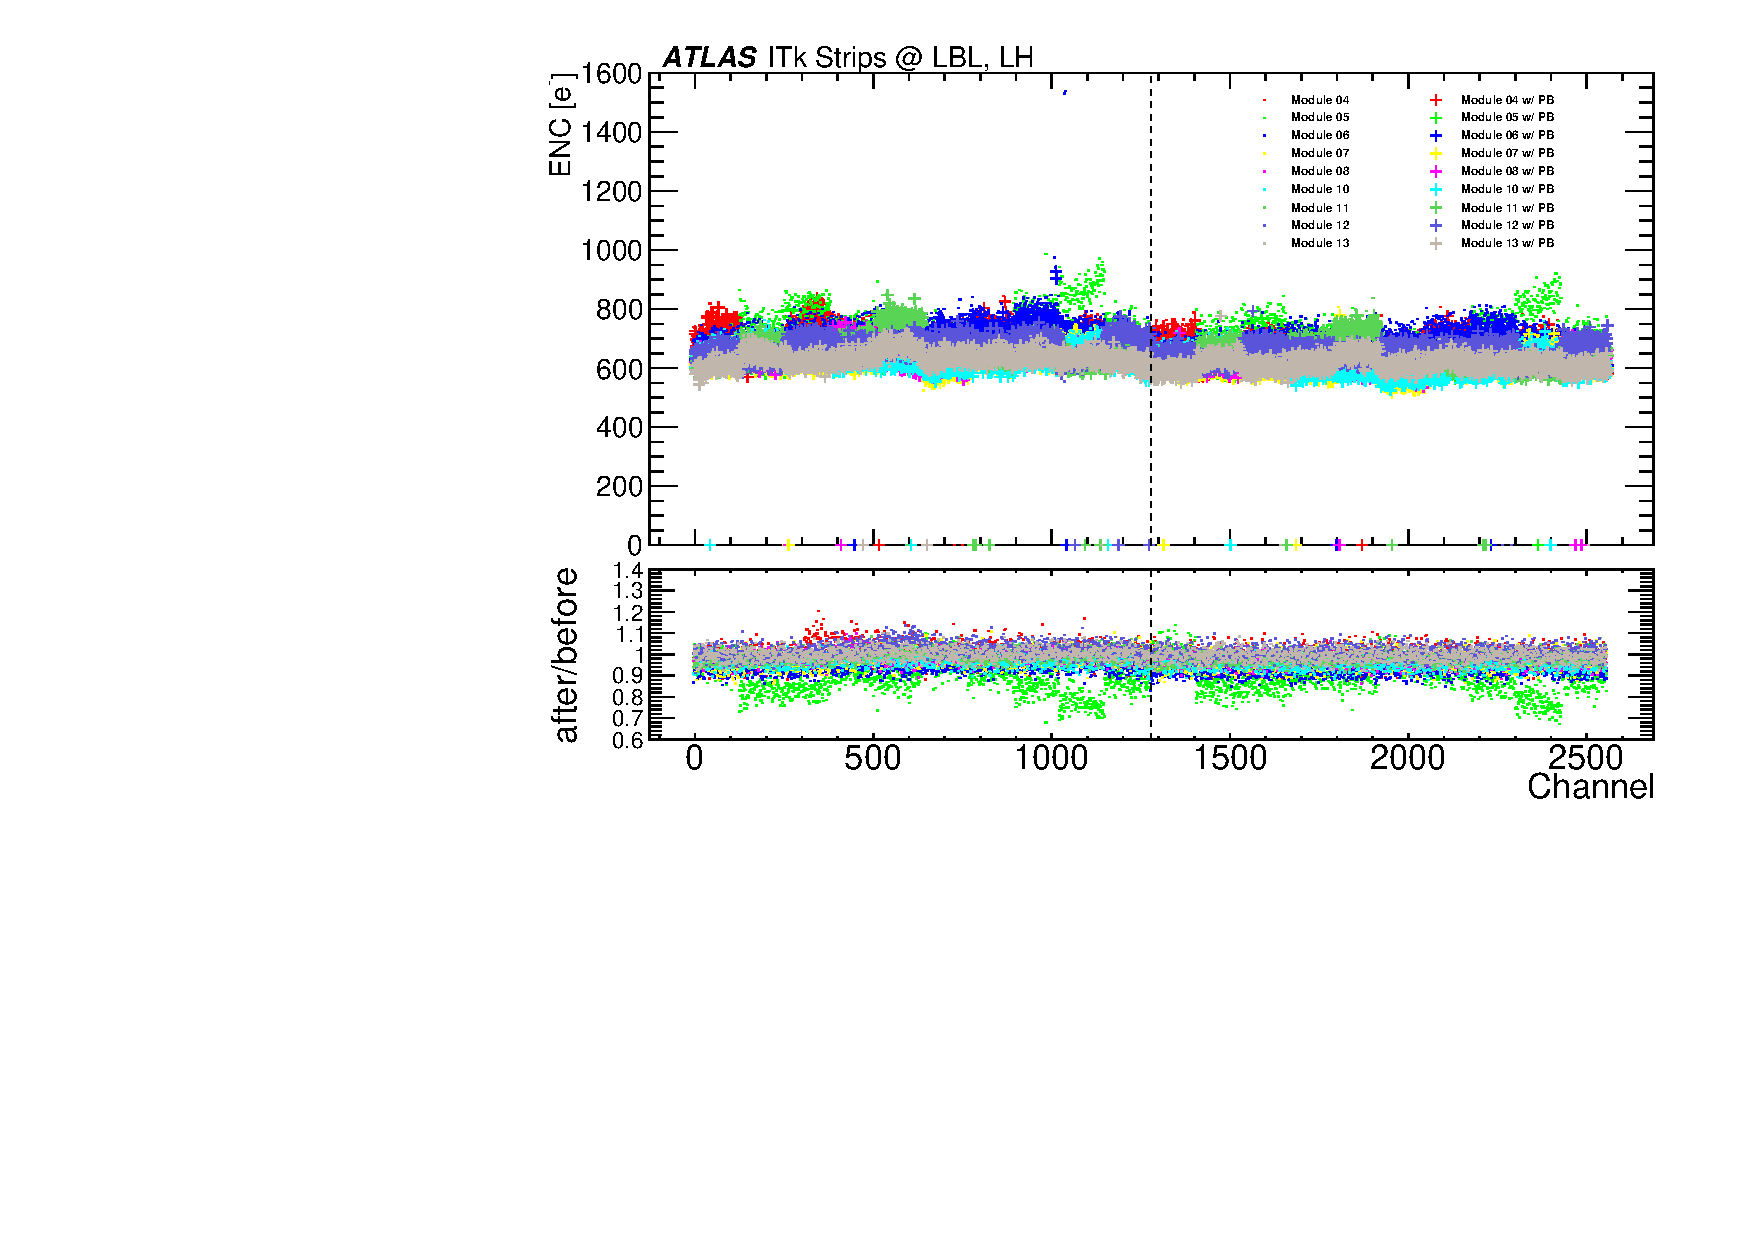
\includegraphics[width=0.65\textwidth, angle=-90]{fig/LH_noise.pdf} \\
  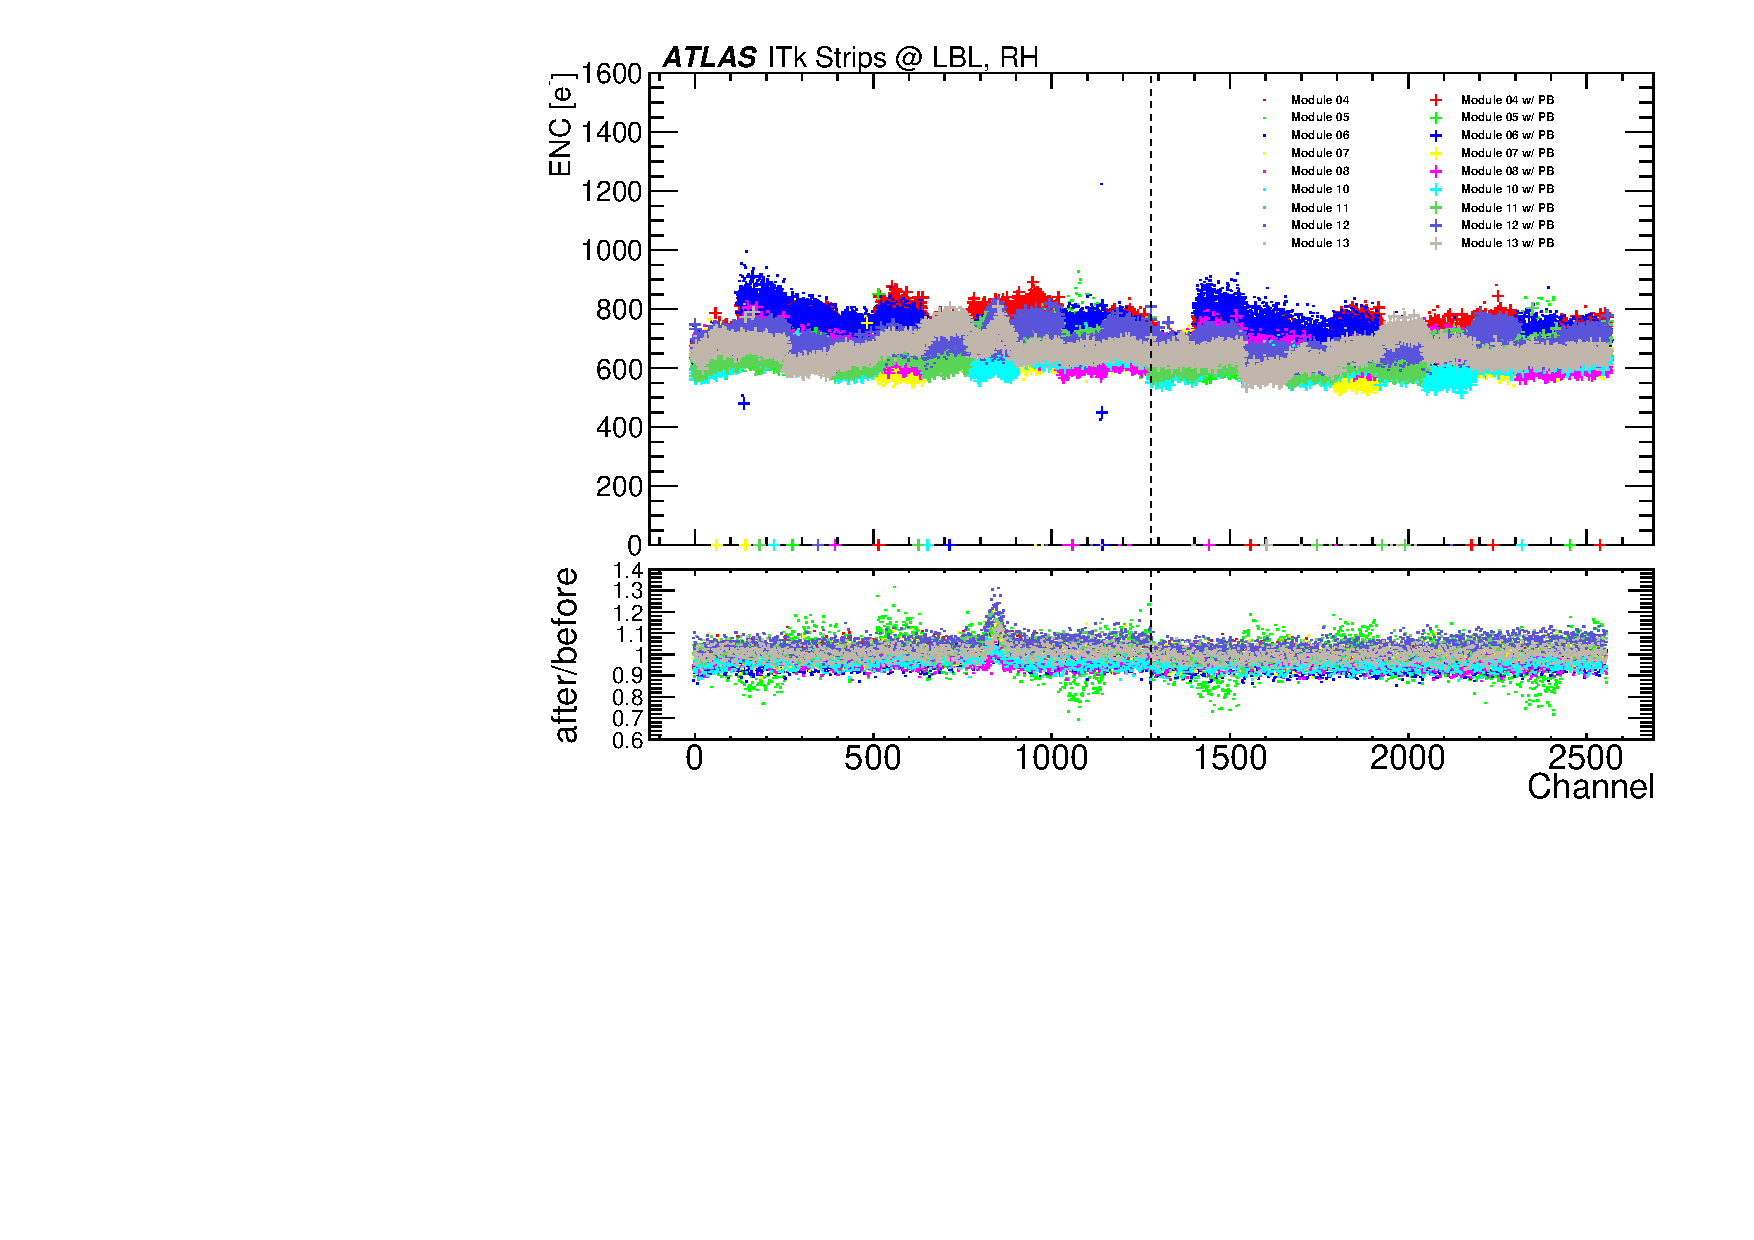
\includegraphics[width=0.65\textwidth, angle=-90]{fig/RH_noise.pdf} 
 \caption{Strips模块输入噪声,上图对应左手Hybrid (LH),下图对应右手Hybrid (RH), 点线为粘合PB之前,'+'为粘合PB之后,每图底部为粘合PB之后与之前的噪声之比。
 总体上比例在1附近,但因为每次实际测试时,环境参数并不一致,所以不能够表明粘合PB之后噪声一定增加或者减少了。}
 \label{fig:strips_testing_noise}
\end{figure}
\begin{figure}[h]
\centering
\begin{subfigure}[b]{0.45\textwidth}
\centering
 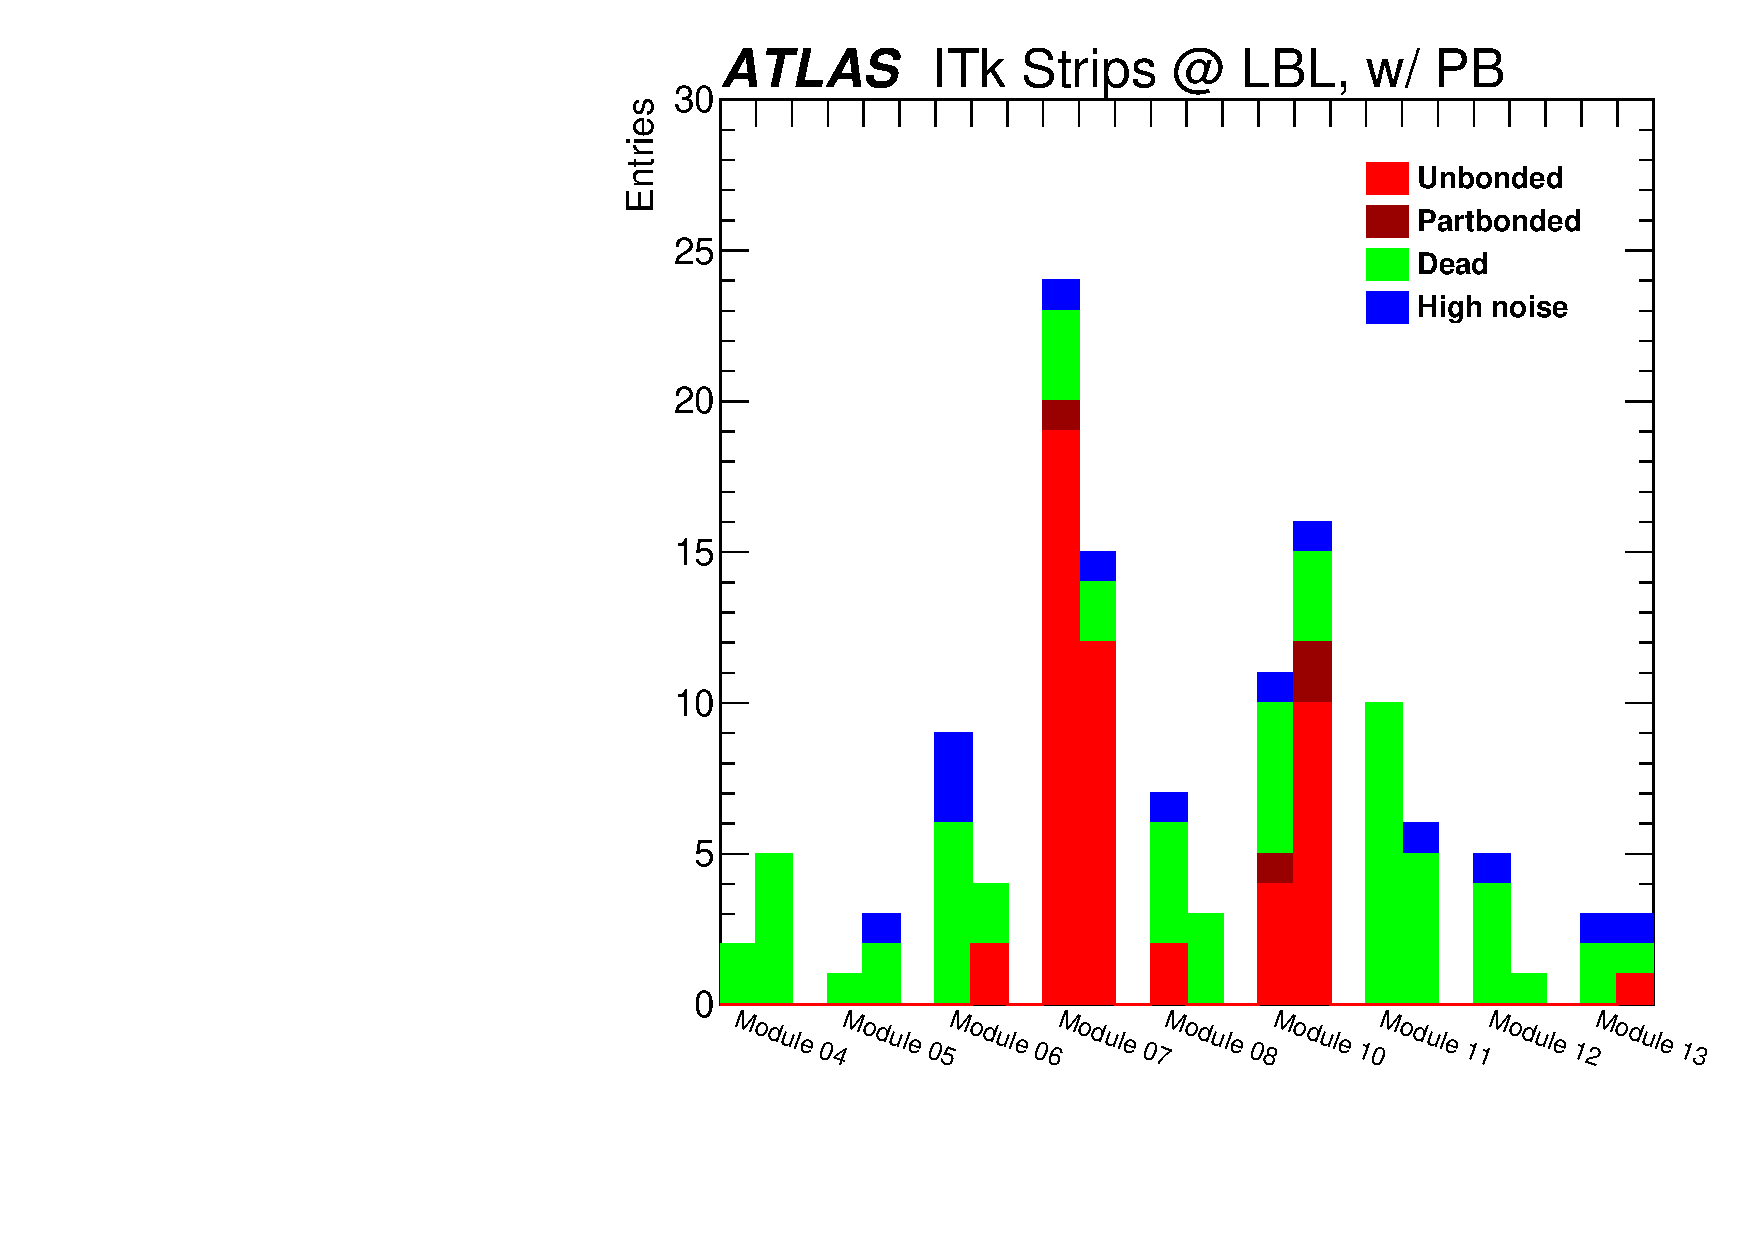
\includegraphics[width=0.9\textwidth,angle=-90]{fig/Hists_Bad_wPB.pdf}
 \caption{}
\end{subfigure}
\begin{subfigure}[b]{0.45\textwidth}
\centering
 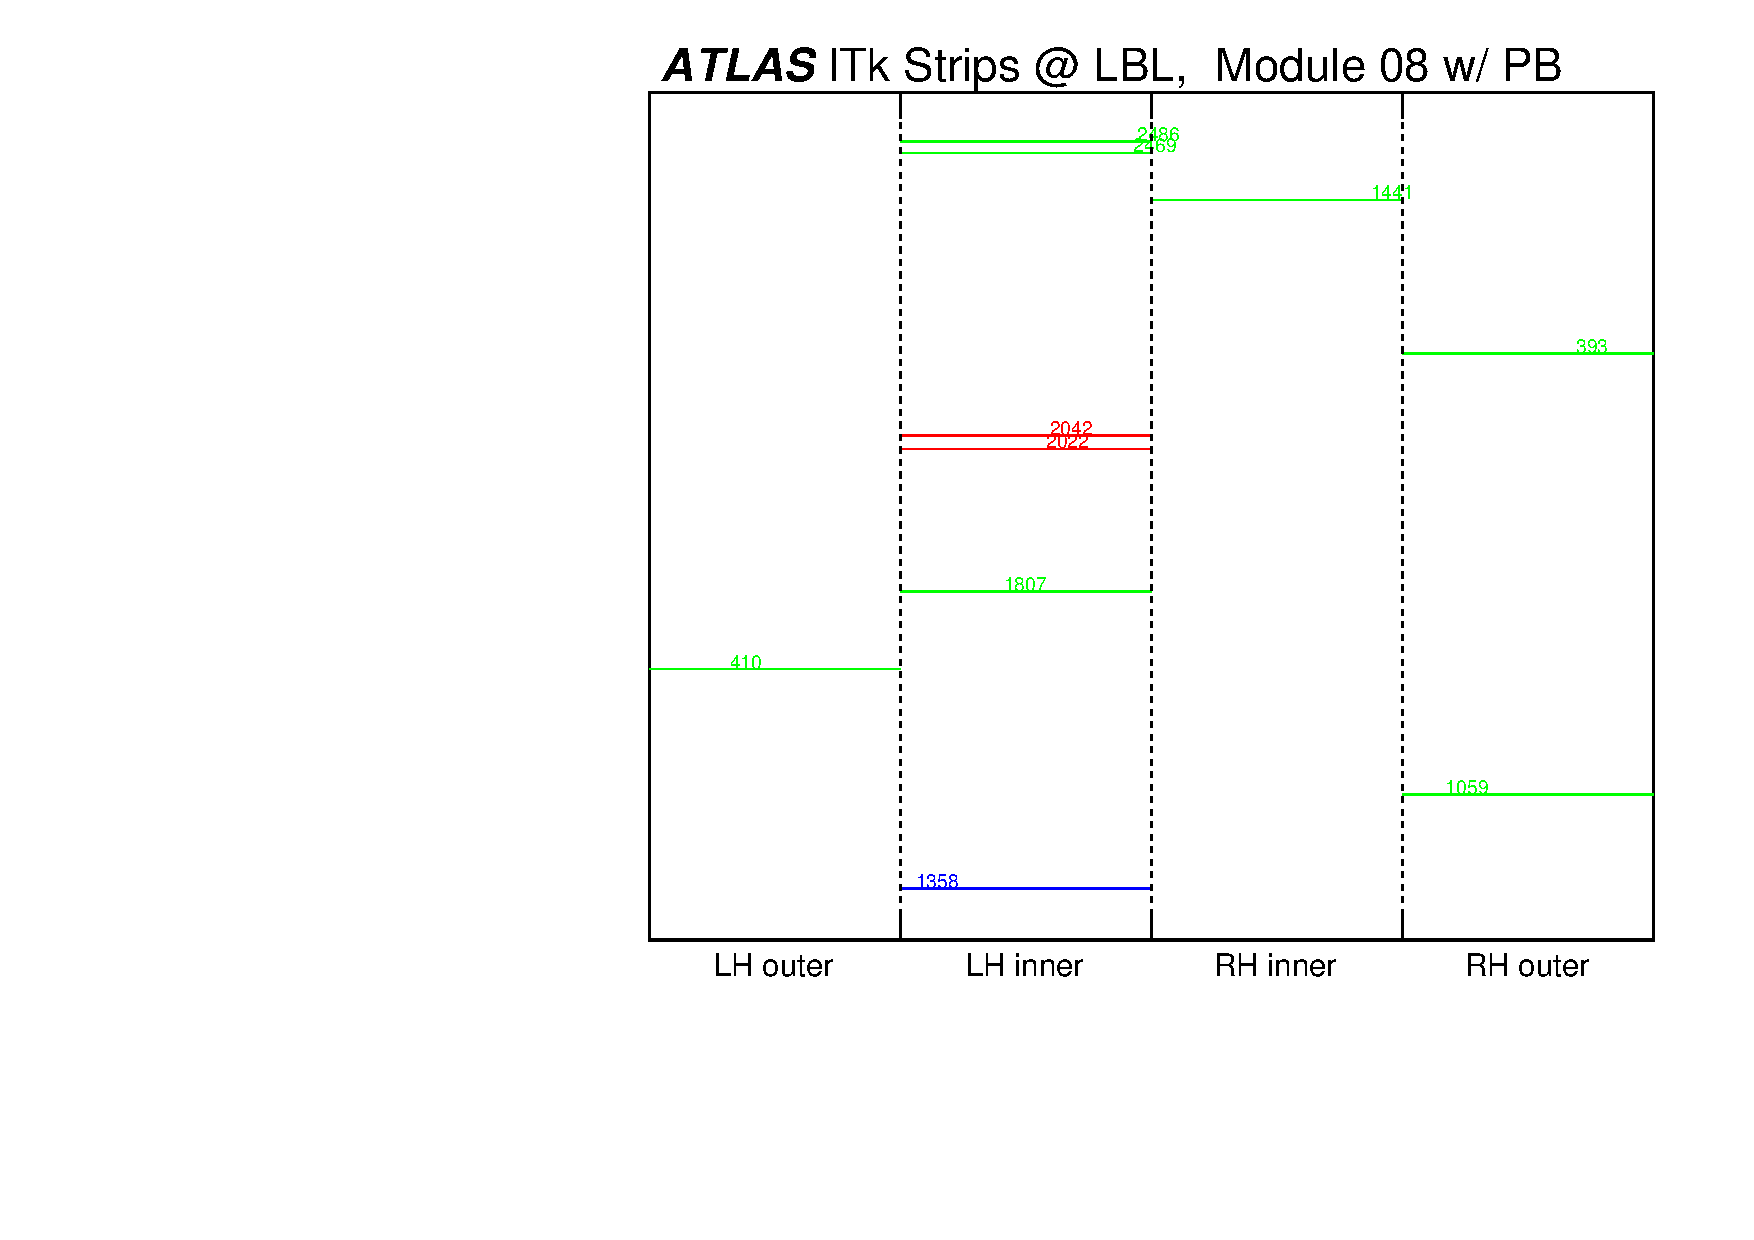
\includegraphics[width=0.9\textwidth,angle=-90]{fig/BadDistr_LBL-EL-08_wPB.pdf}
 \caption{}
\end{subfigure}
\caption{(a)为测试模块strip整体不良率;(b)为LBL-EL-08模块不良strip在传感器上的分布情况。}
\label{fig:strips_bad_dist}
\end{figure}

\subsection{ITk预期寻迹性能}
相比目前的内部径迹探测器,ITk具有更低的物质量\footnote{目前研究显示材料预算在TDR被低估,这些预期结果也许过于乐观,全新的估计正在进行。},其具有更高的寻迹效率和分辨。
径迹重建从种子(seed)开始,所谓的seed是三个空间点。
在ITk的前期研究中,只考虑了两种seed,全部由Pixel着火点组成的PPP,全部由Strips着火点组成的SSS。
图\ref{fig:ITk_seeds}展示seeds随\abseta 分布,整体而言,PPP比SSS数目高一个量级。
联合拟合PPP与SSS,并消除掉重复着火点,同时满足一系列条件,即得到最终的径迹。
图\ref{fig:ITk_tracking_eff}展示径迹重建效率随$\eta$分布,可达90\%。
值得一提的是,由于径迹重建性能的提高,相比于\RunTwo ,电子电荷误判率下降,见图\ref{fig:ITk_ele_qmisid}。
\begin{figure}[h]
\centering
 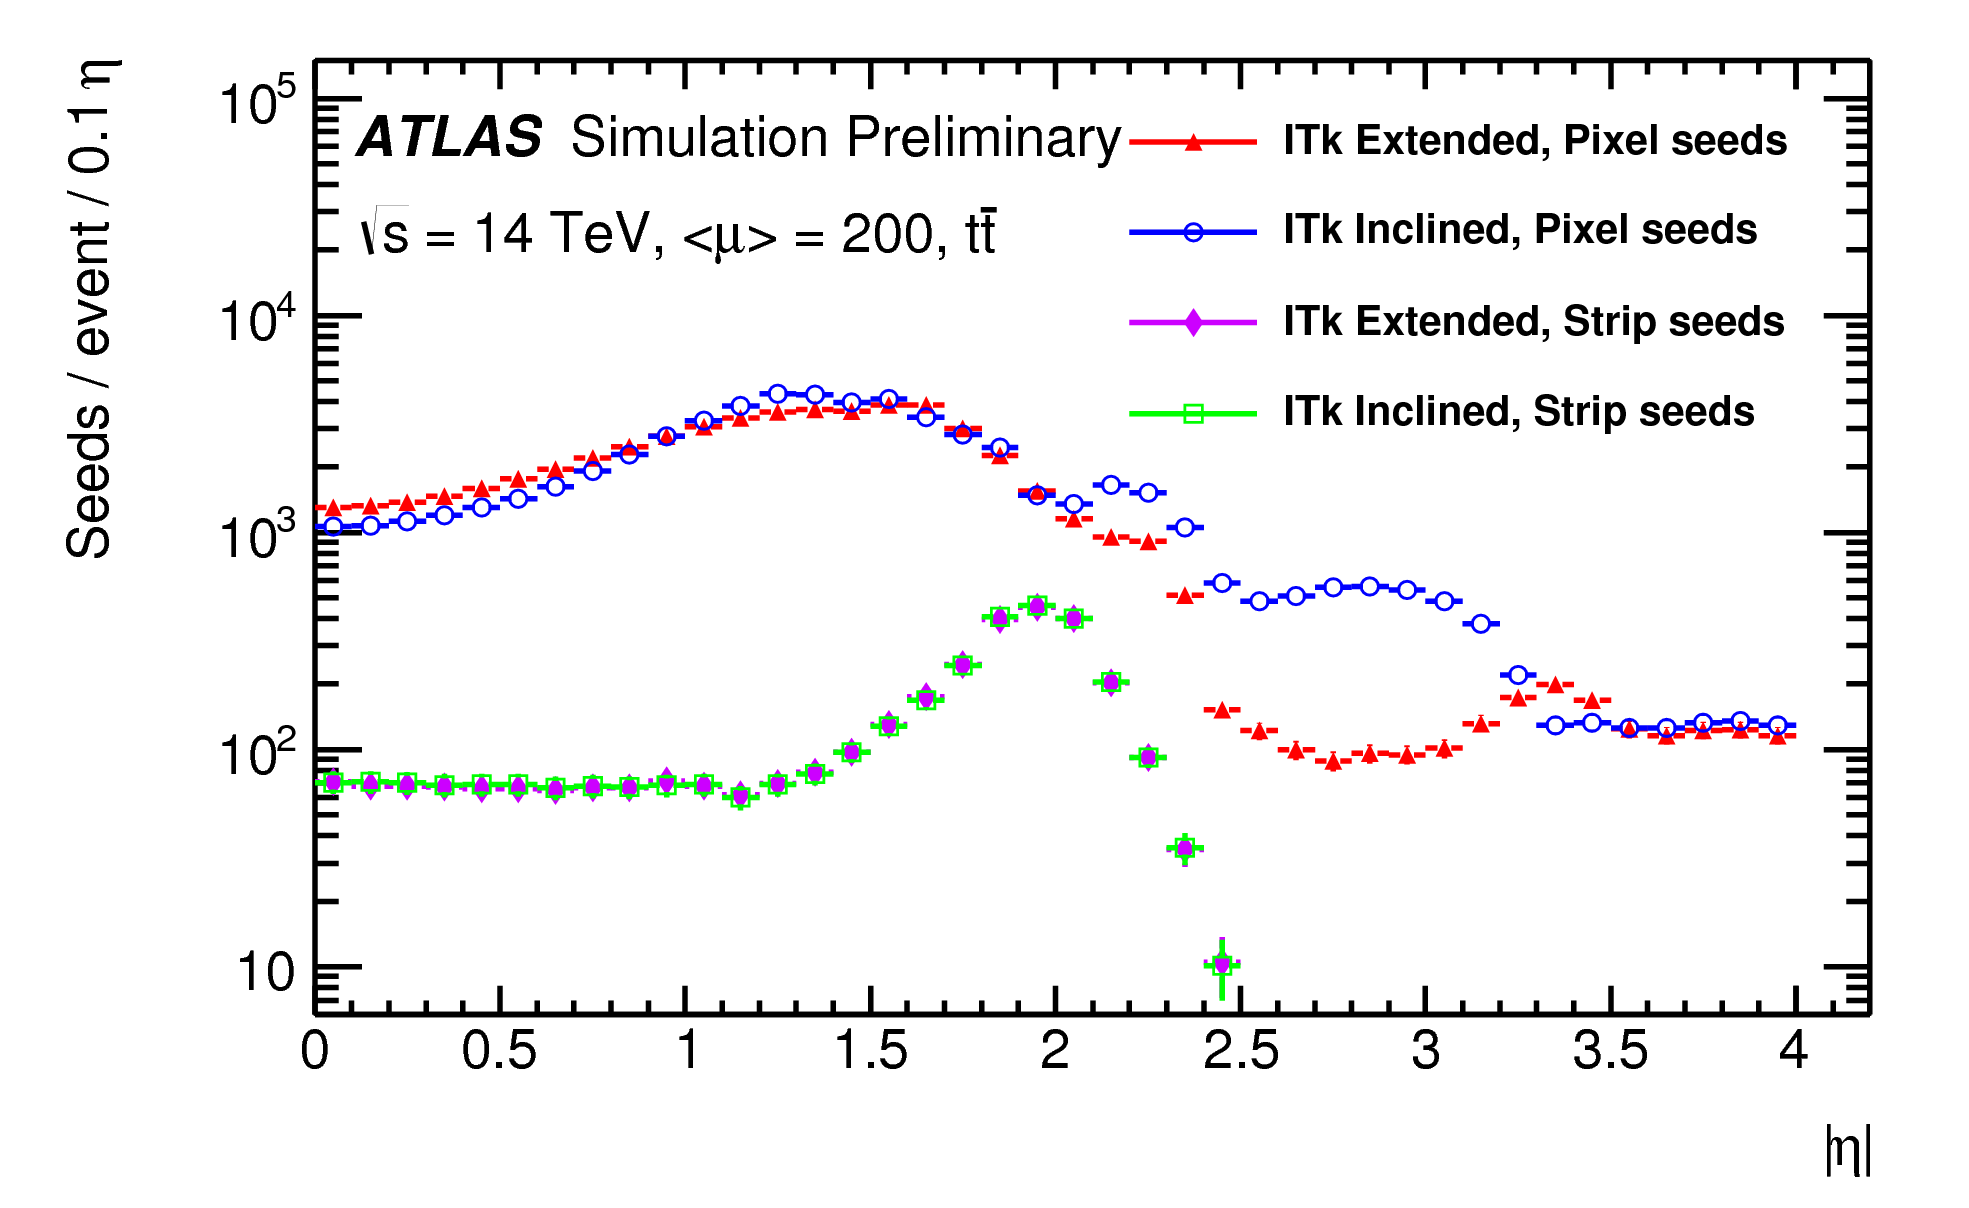
\includegraphics[width=0.85\textwidth]{fig/ITk_seeds.png}
 \caption{ITk seeds随\abseta 分布%\footnote{在ITk研究前期,有两种布局,最后选用Inclined作为baseline}
\cite{seeds_ITk}。}
 \label{fig:ITk_seeds}
\end{figure}
\begin{figure}[h]
\centering
\begin{subfigure}[b]{0.45\textwidth}
\centering
 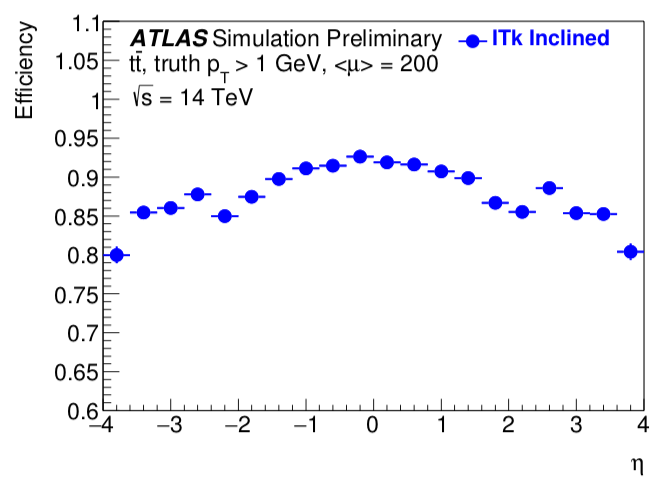
\includegraphics[width=0.9\textwidth]{fig/ITk_tracking_eff_tt.png}
 \caption{}
\end{subfigure}
\begin{subfigure}[b]{0.45\textwidth}
\centering
 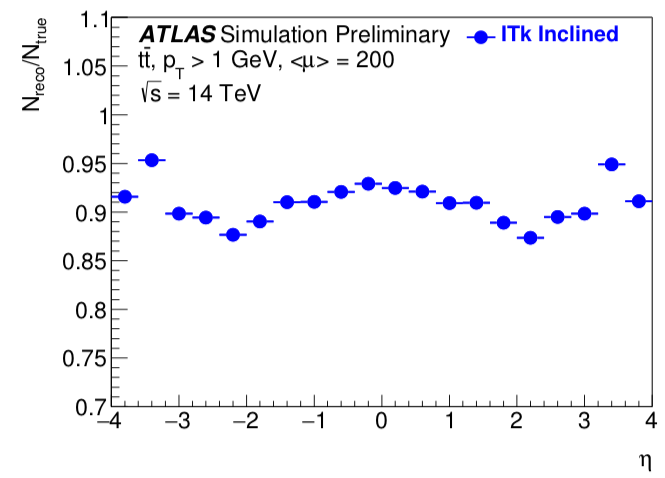
\includegraphics[width=0.9\textwidth]{fig/ITk_tracking_eff_ratio.png}
 \caption{}
\end{subfigure}
\caption{(a) 径迹重建效率随$\eta$分布(matching criteria);(b) 重建径迹与真实粒子之比随$\eta$分布(no matching criteria)。\cite{ATL-PHYS-PUB-2016-025}}
\label{fig:ITk_tracking_eff}
\end{figure}
\begin{figure}[h]
\centering
\begin{subfigure}[b]{0.45\textwidth}
\centering
 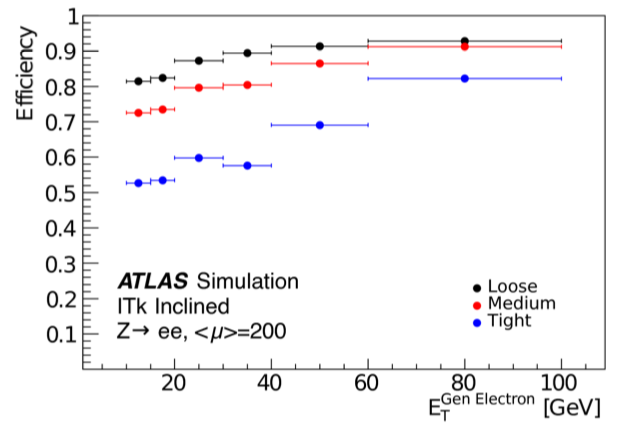
\includegraphics[width=0.9\textwidth]{fig/ITk_ele_qmisid1.png}
 \caption{}
\end{subfigure}
\begin{subfigure}[b]{0.45\textwidth}
\centering
 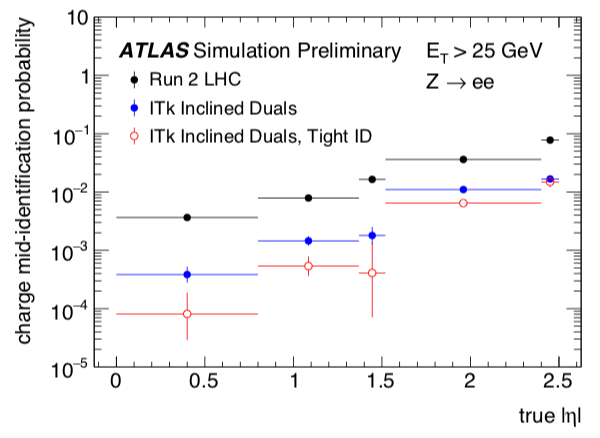
\includegraphics[width=0.9\textwidth]{fig/ITk_ele_qmisid2.png}
 \caption{}
\end{subfigure}
\caption{(a) 不同工作点的电子鉴别效率随\et 分布;(b)电子电荷误判率随\abseta 分布。\cite{ATL-PHYS-PUB-2019-005}}
\label{fig:ITk_ele_qmisid}
\end{figure}

